% БҮЛЭГ 4: ХЭРЭГЖИЛТ БА ТУРШИЛТ
\chapter{ХЭРЭГЖИЛТ БА ТУРШИЛТ}
\label{Chapter4}
\pagecolor{white}

%===============================================================
\section{4.1 Хөгжүүлэлтийн орчин}

Системийг хөгжүүлэхэд ашигласан хэрэгслүүдийг Хүснэгт~\ref{tab:devtools} дээр харуулав.

\begin{table}[htbp]
\caption{Хөгжүүлэлтийн хэрэгслүүд}
\label{tab:devtools}
\centering
\begin{tabularx}{0.85\textwidth}{|>{\bfseries}X|X|}
\hline
\rowcolor{TableHeader}\textcolor{white}{\textbf{Хэрэгсэл}}
  & \textcolor{white}{\textbf{Зориулалт}} \\ \hline
Visual Studio Code & Кодын засварлагч \\ \hline
Postman            & API туршилт \\ \hline
pgAdmin 4          & Өгөгдлийн сангийн удирдлага \\ \hline
Android Studio     & Android эмулятор \\ \hline
Xcode              & iOS симулятор \\ \hline
Git + GitHub       & Хувилбарын удирдлага \\ \hline
Jest + Supertest   & Нэгж болон интеграцийн тест \\ \hline
Apache JMeter      & Ачааллын туршилт \\ \hline
OWASP ZAP          & Аюулгүй байдлын туршилт \\ \hline
\end{tabularx}
\end{table}

%===============================================================
\section{4.2 Системийн бүрэлдэхүүн хэсгүүдийн хэрэгжилтийн тодорхойлолт}

\subsection{4.2.1 QR Кодын Механизм}

QR кодын URL бүтэц нь дараах мэдээллийг агуулна:

\begin{equation}
\texttt{https://app.restaurant.mn/order?t=\{tableToken\}\&r=\{restaurantId\}}
\end{equation}

\textbf{t параметр:} JWT token бөгөөд tableId ба restaurantId-г шифрлэн агуулна.
24 цагийн хүчинтэй хугацаатай. Серверийн нууц түлхүүрээр гарын үсэг зурсан тул
хуурамчаар үүсгэх боломжгүй.

\textbf{r параметр:} Рестораны нийтийн UUID. Шифрлэх шаардлагагүй.

QR кодыг ширээн дэлгэцэнд байрлуулахдаа: 5$\times$5 см хэмжээнд хэвлэх,
ламинат хийж бохирдлоос хамгаалах, 300 DPI нягтралтай зураг ашиглах.

\subsection{4.2.2 Session Удирдлагын Механизм}

QR уншихад сервер шинэ Session ID (UUID) үүсгэнэ. Session ID нь:
\begin{itemize}
    \item Нэг зочны нэг очилтыг тэмдэглэнэ;
    \item Захиалга болон orders хүснэгтийг холбоно;
    \item WebSocket room-ийн нэр болно (\texttt{session\_\{id\}});
    \item Зочин гарч дахин ороход шинэ session үүснэ.
\end{itemize}

\subsection{4.2.3 Захиалгын Статусын Дарааллын Хяналт}

\begin{figure}[htbp]
\centering
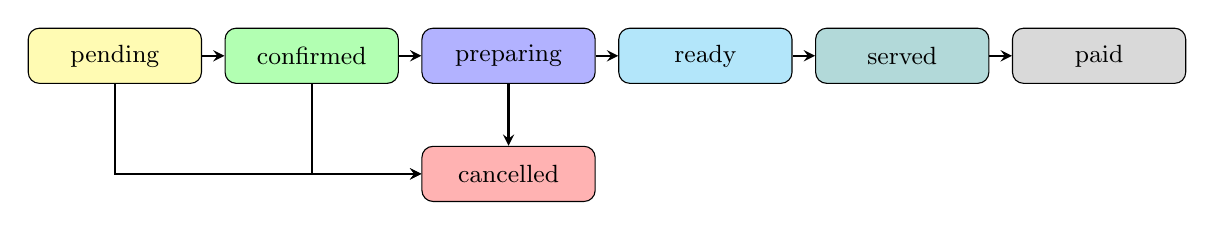
\begin{tikzpicture}[
    state/.style={rectangle, draw, rounded corners, minimum width=2.2cm, minimum height=0.7cm, align=center, font=\small},
    arrow/.style={->, >=stealth, thick}
]
\node[state, fill=yellow!30]  (p) at (0, 0)    {pending};
\node[state, fill=green!30]   (c) at (2.5, 0)  {confirmed};
\node[state, fill=blue!30]    (pr) at (5, 0)   {preparing};
\node[state, fill=cyan!30]    (r) at (7.5, 0)  {ready};
\node[state, fill=teal!30]    (s) at (10, 0)   {served};
\node[state, fill=gray!30]    (pd) at (12.5, 0){paid};
\node[state, fill=red!30]     (cn) at (5, -1.5){cancelled};

\draw[arrow] (p) -- (c);
\draw[arrow] (c) -- (pr);
\draw[arrow] (pr) -- (r);
\draw[arrow] (r) -- (s);
\draw[arrow] (s) -- (pd);
\draw[arrow] (p) |- (cn);
\draw[arrow] (c) |- (cn);
\draw[arrow] (pr) -- (cn);
\end{tikzpicture}
\caption{Захиалгын статусын шилжилтийн диаграм}
\label{fig:status}
\end{figure}

\subsection{4.2.4 WebSocket Өрөөний (Room) Удирдлага}

Socket.IO rooms нь хэрэглэгчдийг логикийн бүлгүүдэд хуваах арга юм:

\begin{itemize}
    \item \texttt{restaurant\_\{id\}} — Бүх ажилтан (цайчин, тогооч, менежер);
    \item \texttt{kitchen\_\{id\}} — Зөвхөн тогоочид;
    \item \texttt{waiters\_\{id\}} — Зөвхөн цайчид;
    \item \texttt{session\_\{id\}} — Нэг зочны нэг очилт.
\end{itemize}

Захиалга ирэхэд \texttt{restaurant\_\{id\}} room-д мэдэгдэл цацах нь цайчин,
тогооч, менежер бүгдэд нэгэн зэрэг хүрэх боломжийг хангана.

%===============================================================
\section{4.3 Системийг ажиллуулах журам}

\subsection{4.3.1 Серверийн тохиргоо}

\begin{enumerate}
    \item \textbf{Орчны тохиргоо:} \texttt{.env} файлд DATABASE\_URL, JWT\_SECRET,
          TABLE\_TOKEN\_SECRET, PORT зэрэг хувьсагчдыг тохируулна;
    \item \textbf{Өгөгдлийн сангийн схем:} \texttt{pnpm run db:push} командаар
          Drizzle schema-г PostgreSQL-д apply хийнэ;
    \item \textbf{Сервер эхлүүлэх:} \texttt{pnpm run dev} командаар хөгжүүлэлтийн
          горимд эхлүүлнэ.
\end{enumerate}

\subsection{4.3.2 Мобайл аппликейшн тохиргоо}

\begin{enumerate}
    \item Expo Go аппликейшнийг iOS/Android дээр суулгана;
    \item \texttt{pnpm run mobile} командаар Expo dev server эхлүүлнэ;
    \item QR код уншуулан Expo Go-оор аппликейшн нээнэ.
\end{enumerate}

\subsection{4.3.3 Анхны тохиргооны дараалал}

\begin{enumerate}
    \item Администраторын бүртгэл үүсгэх;
    \item Рестораны мэдээлэл нэмэх;
    \item Ширээ нэмэж QR код үүсгэх, хэвлэж ширээн дэлгэцэнд байрлуулах;
    \item Цэсний ангилал болон хоолнуудыг оруулах;
    \item Ажилтан бүрийн бүртгэл үүсгэж үүрэг тохируулах.
\end{enumerate}

%===============================================================
\section{4.4 Туршилтын аргачлал}

Туршилт нь Улаанбаатар хотын 3 рестораны 2 долоо хоногийн турш явагдав.
\textbf{Квазитуршилтын дизайн} (quasi-experimental design) ашигласан:
нэг долоо хоног уламжлалт аргаар, дараагийн долоо хоногт QR мобайл системээр
нийт 1,240 захиалгыг бүртгэв.

\begin{table}[htbp]
\caption{Туршилтын ресторануудын мэдээлэл}
\label{tab:restaurants}
\centering
\begin{tabularx}{\textwidth}{|>{\bfseries}X|Z|Z|X|}
\hline
\rowcolor{TableHeader}\textcolor{white}{\textbf{Ресторан}}
  & \textcolor{white}{\textbf{Ширээний тоо}}
  & \textcolor{white}{\textbf{Хэрэглэгч/өдөр}}
  & \textcolor{white}{\textbf{Мэргэшил}} \\ \hline
Ресторан А (Сүхбаатар дүүрэг) & 40 & 120--180 & Монгол, Европ хоол \\ \hline
Ресторан Б (Баянзүрх дүүрэг)  & 25 & 80--120  & Монгол хоол \\ \hline
Ресторан В (Хан-Уул дүүрэг)   & 60 & 200--280 & Олон улсын хоол \\ \hline
\end{tabularx}
\end{table}

%===============================================================
\section{4.5 Туршилтын үр дүн}

\subsection{4.5.1 Захиалгын Хугацааны Харьцуулалт}

\begin{table}[htbp]
\caption{Захиалгын хугацааны харьцуулалт (секунд)}
\label{tab:time}
\centering
\begin{tabularx}{\textwidth}{|X|Z|Z|Z|}
\hline
\rowcolor{TableHeader}\textcolor{white}{\textbf{Алхам}}
  & \textcolor{white}{\textbf{Уламжлалт}}
  & \textcolor{white}{\textbf{QR систем}}
  & \textcolor{white}{\textbf{Бууралт}} \\ \hline
Цэс авах/нээх           & 185 сек & 5 сек  & 97.3\% \\ \hline
Захиалга бичих           & 78 сек  & 52 сек & 33.3\% \\ \hline
Кухинд дамжуулах         & 45 сек  & 2 сек  & 95.6\% \\ \hline
\rowcolor{yellow!20}\textbf{Нийт дундаж} & \textbf{308 сек} & \textbf{59 сек} & \textbf{80.8\%} \\ \hline
\end{tabularx}
\end{table}

\subsection{4.5.2 Захиалгын Алдааны Харьцуулалт}

\begin{table}[htbp]
\caption{Захиалгын алдааны харьцуулалт}
\label{tab:error}
\centering
\begin{tabularx}{0.85\textwidth}{|X|Z|Z|}
\hline
\rowcolor{TableHeader}\textcolor{white}{\textbf{Алдааны төрөл}}
  & \textcolor{white}{\textbf{Уламжлалт (\%)}}
  & \textcolor{white}{\textbf{QR систем (\%)}} \\ \hline
Буруу хоол захиалагдсан   & 14.2 & 1.1 \\ \hline
Хэмжээ/тоо буруу           & 5.3  & 0.6 \\ \hline
Тусгай хүсэлт алдагдсан   & 3.8  & 0.3 \\ \hline
\rowcolor{yellow!20}\textbf{Нийт}           & \textbf{23.3} & \textbf{2.0} \\ \hline
\end{tabularx}
\end{table}

\subsection{4.5.3 WebSocket Мэдэгдлийн Хоцролт}

100 зэрэг захиалгын нөхцөлд Socket.IO мэдэгдлийн хоцролтыг хэмжсэн үр дүн:

\begin{table}[htbp]
\caption{WebSocket мэдэгдлийн гүйцэтгэл}
\label{tab:latency}
\centering
\begin{tabularx}{0.6\textwidth}{|X|Z|}
\hline
\rowcolor{TableHeader}\textcolor{white}{\textbf{Метрик}}
  & \textcolor{white}{\textbf{Утга}} \\ \hline
Дундаж хоцролт         & 42 ms \\ \hline
Медиан                 & 38 ms \\ \hline
95-р перцентиль        & 87 ms \\ \hline
99-р перцентиль        & 134 ms \\ \hline
Хамгийн их             & 210 ms \\ \hline
Амжилтын хувь          & 99.7\% \\ \hline
\end{tabularx}
\end{table}

\subsection{4.5.4 Хэрэглэгчийн Сэтгэл Ханамжийн Үнэлгээ}

60 зочин болон 18 ажилтнаас авсан судалгааны үр дүн (1--5 оноо):

\begin{table}[htbp]
\caption{Зочдын сэтгэл ханамжийн үнэлгээ ($n=60$)}
\label{tab:sat}
\centering
\begin{tabularx}{0.85\textwidth}{|X|Z|}
\hline
\rowcolor{TableHeader}\textcolor{white}{\textbf{Хэмжигдэхүүн}}
  & \textcolor{white}{\textbf{Дундаж оноо}} \\ \hline
QR уншуулах хялбар байдал      & 4.6 \\ \hline
Цэс ойлгомжтой байдал          & 4.4 \\ \hline
Захиалга өгөх хялбар байдал    & 4.5 \\ \hline
Статусын мэдэгдэл хэрэгтэй байдал & 4.8 \\ \hline
\rowcolor{yellow!20}\textbf{Нийт сэтгэл ханамж} & \textbf{4.5} \\ \hline
\end{tabularx}
\end{table}

Зочдын \textbf{91.7\%} (55/60) нь ``Та энэ системийг ашигладаг ресторанд
дахин ирэх үү?'' гэсэн асуултад \textbf{``Тийм''} гэж хариулсан.

\subsection{4.5.5 Ачааллын Туршилт}

Apache JMeter ашиглан 200 зэрэг хэрэглэгчийн 10 минутын туршилтын үр дүн:

\begin{table}[htbp]
\caption{API endpoint-уудын гүйцэтгэлийн туршилт}
\label{tab:loadtest}
\centering
\begin{tabularx}{\textwidth}{|X|Z|Z|Z|}
\hline
\rowcolor{TableHeader}\textcolor{white}{\textbf{Endpoint}}
  & \textcolor{white}{\textbf{Дундаж хариу}}
  & \textcolor{white}{\textbf{95th\%}}
  & \textcolor{white}{\textbf{Алдааны\%}} \\ \hline
GET /api/tables/:id/menu   & 67 ms  & 112 ms & 0\%   \\ \hline
POST /api/orders           & 89 ms  & 165 ms & 0.2\% \\ \hline
PATCH /api/orders/:id/status & 54 ms & 98 ms & 0\%  \\ \hline
WebSocket event            & 42 ms  & 87 ms  & 0.3\% \\ \hline
\end{tabularx}
\end{table}

\subsection{4.5.6 Нэгж болон Интеграцийн Туршилт}

\begin{table}[htbp]
\caption{Нэгж туршилтын үр дүн}
\label{tab:unittest}
\centering
\begin{tabularx}{0.85\textwidth}{|X|Z|Z|Z|}
\hline
\rowcolor{TableHeader}\textcolor{white}{\textbf{Туршилтын хэсэг}}
  & \textcolor{white}{\textbf{Нийт}}
  & \textcolor{white}{\textbf{Амжилт}}
  & \textcolor{white}{\textbf{Хувь}} \\ \hline
Auth service     & 34  & 34  & 100\% \\ \hline
Menu service     & 28  & 28  & 100\% \\ \hline
Order service    & 42  & 41  & 97.6\% \\ \hline
Table service    & 18  & 18  & 100\% \\ \hline
\rowcolor{yellow!20}\textbf{Нийт} & \textbf{122} & \textbf{121} & \textbf{99.2\%} \\ \hline
\end{tabularx}
\end{table}

%===============================================================
\section{4.6 Аюулгүй байдлын туршилт}

OWASP ZAP хэрэгсэл ашиглан автоматжсан аюулгүй байдлын туршилт хийв:

\begin{table}[htbp]
\caption{Аюулгүй байдлын туршилтын үр дүн}
\label{tab:security}
\centering
\begin{tabularx}{\textwidth}{|X|X|Z|}
\hline
\rowcolor{TableHeader}\textcolor{white}{\textbf{Аюулын төрөл}}
  & \textcolor{white}{\textbf{Туршилтын аргачлал}}
  & \textcolor{white}{\textbf{Үр дүн}} \\ \hline
SQL Injection  & Injection payload оруулах  & Блок болсон \\ \hline
XSS            & HTML/JS тэмдэгт оруулах   & Sanitized \\ \hline
CSRF           & Token-гүй хүсэлт          & 401 Rejected \\ \hline
Brute Force    & 6+ буруу нэвтрэлт         & Rate limit \\ \hline
Broken Auth    & Хүчингүй JWT token         & 401 Rejected \\ \hline
IDOR           & Өөр session-д хандах       & 403 Forbidden \\ \hline
\end{tabularx}
\end{table}

%===============================================================
\section{4.7 Хэлэлцүүлэг}

\textbf{Захиалгын хурд:} QR системийг нэвтрүүлснээр нийт захиалгын хугацаа 80.8\%
буурсан нь Kim нар \cite{kim2023}-ын 64\%, Zhang болон Liu \cite{zhang2022}-ын 2.3 дахин
хурдасгалын дүгнэлттэй нийцэж, Монголын нөхцөлд ч ижил нөлөө гарсныг нотолно.

\textbf{Алдааны бууралт:} 23.3\%-аас 2.0\%-д буурсан алдааны өөрчлөлт нь статистикийн
хувьд ач холбогдолтой ($t(1083) = 47.32$, $p < 0.001$, Cohen's $d = 2.89$). Алдааны
бараг бүх эх үүсвэр нь хүний дамжуулалтын зуучлалтай холбоотой байсан нь дижитал
систем тус зуучлалыг арилгасны үр дүн болов.

\textbf{Хэрэглэгчийн туршлага:} Patel нар \cite{patel2022}-ын хэрэглэгчийн автономи
(захиалгаа өөрөө удирдах чадамж) нь сэтгэл ханамжийн гол хүчин зүйл гэсэн
дүгнэлтийг тус судалгааны чанарын хариу (зочдын 28/60 нь цайчнийг хүлээхгүй
захиалах боломж давуу тал гэсэн) батална.
